\section{Propriedades}\label{sec:props}
As propriedades do material necessários para a simulação são a condutividade
térmica, o calor específico, a densidade, a permeabilidade e a água quimicamente
ligada contina na microestrutura do concreto, conforme apresentadas na Figura
\ref{fig:properties}.

 \begin{figure}[ht]
\centering
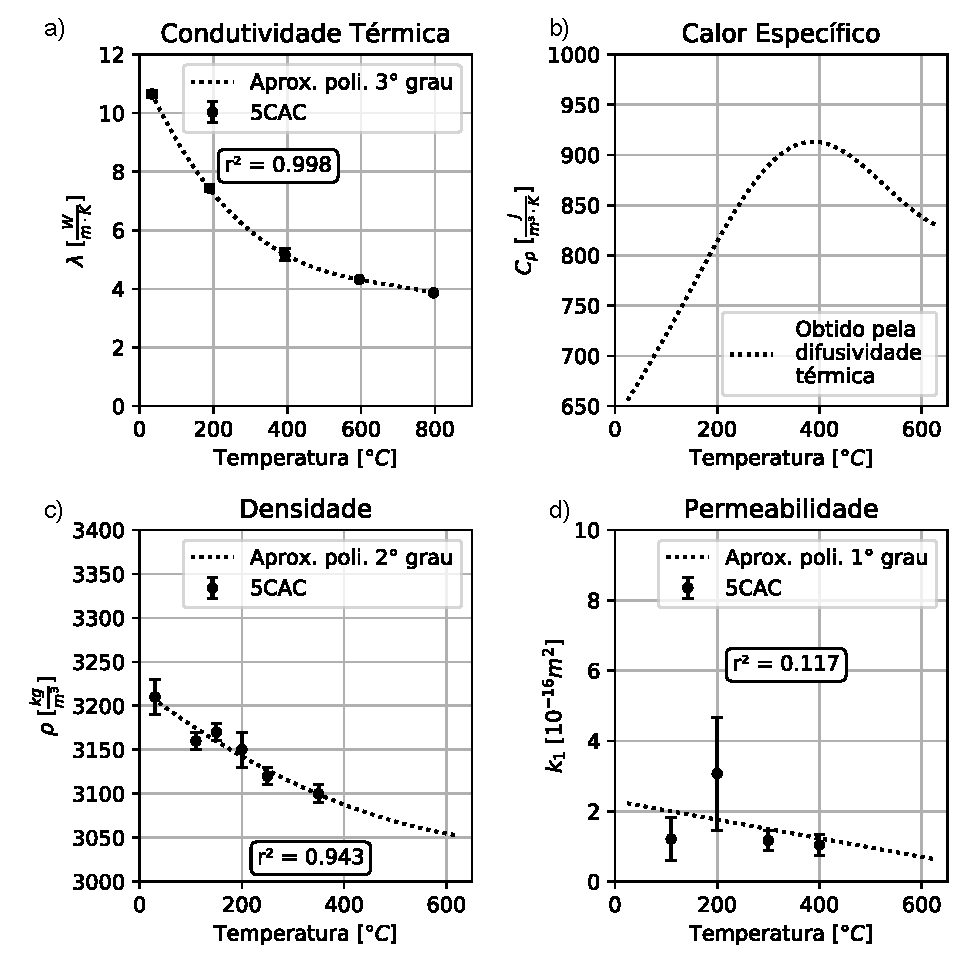
\includegraphics[width=14cm]{./figures/properties.pdf}
\caption{Caracterização da composição de concreto refratário utilizado no
  presente estudo, (a) condutividade térmica, (b) calor específico, (c)
  densidade e permeabilidade (d).  \label{fig:properties}}
\end{figure}

Na faixa avaliada a condutividade térmica decai conforme a temperatura aumenta.
Tal comportamento pode ser aproximado por um polinômio de terceiro grau. Este
comportamento justifica-se pelo aumento da frequência de oscilações dos átomos,
o que diminui o caminho livre médio dos fónons, que são os principais
transportadores de energia térmica até aproximadamente 800$^\degree$C quando o
transporte por radiação começa a predominar \cite{pelissari2017}. A densidade é
reduzida devido a liberação da água físicamente adsorvida, bem como a água
quimicamente ligada. Outro efeito provável é a conversão de fases menos densas
do cimento aluminoso hidratado em fases de maior densidade, o que amplia a
porosidade do material. O calor específico foi calculado a partir da medida de
difusividade térmica, $\alpha = \frac{\lambda}{\rho \ C_p}$, e portanto não é
apresentado o desvio associado. Por fim, a permeabilidade do material apresenta
um desvio padrão muito elevado, e isto reflete no baixo valor de $r^2$ (aqui uma
possível solução seria aumentar o grau do polinômio, porém, seria o equivalente
a realizar um {\it overfitting} uma vez que estaríamos inserindo no modelo um
comportamento que pode ser apenas o produto do erro da medida
\cite{raschka2017}).

 \begin{figure}[ht]
\centering
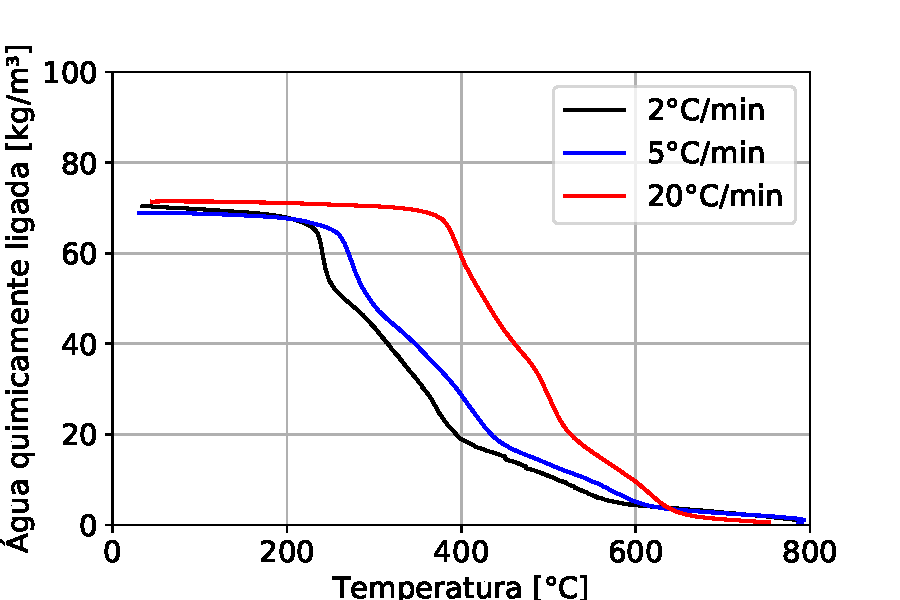
\includegraphics[width=14cm]{./figures/w_d.pdf}
\caption{Água quimicamente ligada por $m^3$ de concreto.  \label{fig:prop_wd}}
\end{figure}

Na Figura \ref{fig:prop_wd} a curva de liberação de água quimicamente ligada é
apresentada. Sua medição é realizada a partir do ensaio de TGA realizado em
amostras previamente secas à 110$^\degree$C por 24 horas. Tal abordagem deve ser
considerada cuidadosamente, uma vez que sua precisão precisa ser investigada mais
a fundo. Uma possível problemática envolvida nessa maneira de medir a água de
desidratação é a formação de fases específicas durante a secagem a
110$^\degree$C, que não estariam presentes em uma secagem do material apenas
curado.



Uma última propriedade fundamental para o modelo são as curvas de sorção
isotérmicas que representam a quantidade de água evaporável (líquida e
adsorvida) no material. Tais medidas são complexas e segundo Baroghen-Bouny
\cite{baroghel2007water}, para se ter medidas confiáveis o método de medida deve
ser o método estacionário com soluções salinas para controle de umidade
relativa. Tais ensaios podem demorar meses até se atingir uma massa de água
adsorvida constante no material. Além da restrição de tempo, há uma notável
histerese quando comparado os comportamentos de sorção e adsorção que devem ser
levados em conta na medida. Como alternativa, há o uso do método dinâmico de
sorção de vapor, utilizado por Fey et al \cite{Fey2016b}, cuja validade das
medidas é limitado até 75\% de umidade relativa. Devido a indisponibilidade de
um equipamento capaz de realizar tais medidas, utilizou-se primeiramente a mesma
curva de sorção de Gong et al \cite{Gong1995a}, em seguida, devido ao desvio
apresentado, tal curva foi ajustada a fim de calibrar os resultados
experimentais com os resultados do modelo.

\section{Ensaios para o \textit{Benchmarking}}
A fim de realizar um benchmark do modelo, é proposto o uso do ensaio
termogravimétrico descrito na Seção \ref{metodologia}. A Figura
\ref{fig:TGA_measured} apresenta os resultados dos ensaios realizados à uma taxa
de 2$^\degree$C/min, 5$^\degree $C/min e 20$^\degree $C/min.

\begin{figure}[ht]
	\centering
	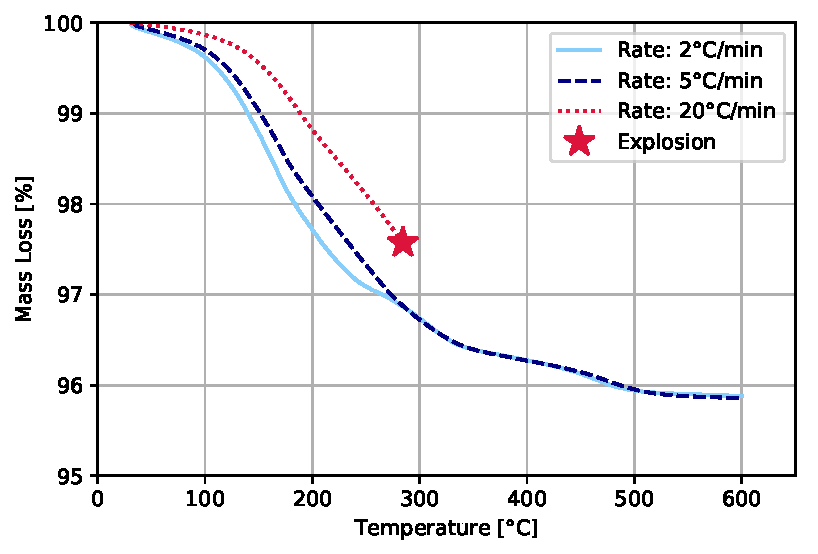
\includegraphics[width=12cm]{./figures/Mass_Loss.pdf}
	\caption{Resultado da perda de massa percentual dos ensaios de TGA realizados
    a taxas de 2$^\degree$ C/min, 5$^\degree$ C/min e 20$^\degree$ C/min.
  \label{fig:TGA_measured}}
\end{figure}

É possível observar que as taxas de perda de massa das amostras aquecidas à
2$^\degree$C/min e 5$^\degree$C/min são similares, com exceção ao intervalo de
100$^\degree$C à 270$^\degree$C (região onde se tem a maior parte de água
fisicamente adsorvida removida do sistema), especialmente após 300$^\degree$C,
assim como mostrado na Figura \ref{fig:prop_wd}. A amostra aquecida à
20$^\degree$C/min apresentou uma menor taxa de perda de massa para baixas
temperaturas, até a ocorrência da explosão por volta dos 290$^\degree$C.

\begin{figure}[ht]
	\centering
	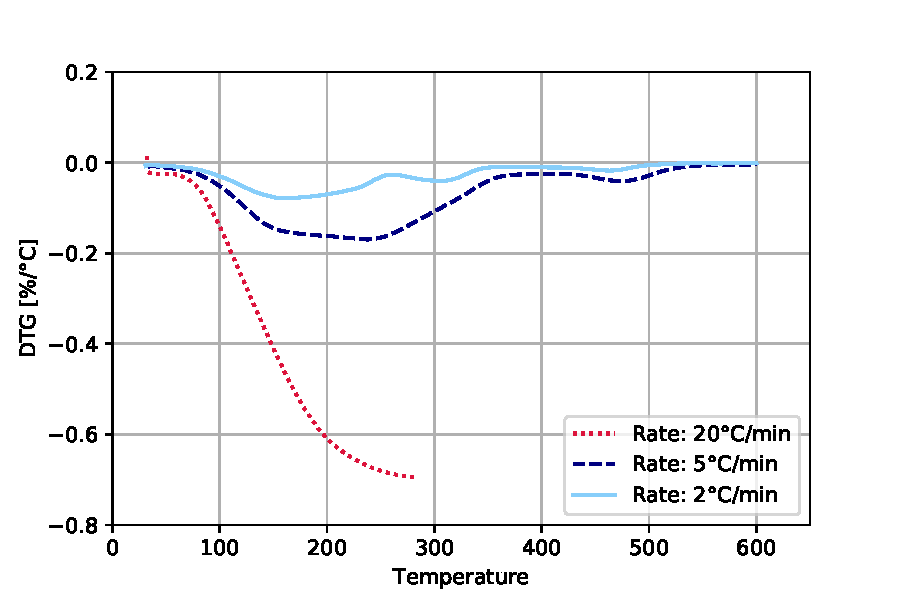
\includegraphics[width=12cm]{./figures/DTG.pdf}
	\caption{Derivada da perda de massa percentual dos ensaios de TGA realizados
    a taxas de 2$^\degree$ C/min, 5$^\degree$ C/min e 20$^\degree$ C/min.
  \label{fig:DTG_measured}}
\end{figure}

A Figura \ref{fig:DTG_measured} apresenta os dados da derivada da curva de perda
de massa com respeito a temperatura. É possível observar que para a curva obtida
a partir do ensaio aquecido à 2$^\degree$C/min existem três picos distintos,
um em torno de 150$^\degree$C, outro em torno de 300$^\degree$C e o último em
torno de 475$^\degree$C. Tais picos podem estar associados com o regime de
evaporação e ebulição da água fisicamente adsorvida, e com as diferentes reações
de desidratação das fases de aluminato de cálcio hidratados
\cite{da2015refractory}.

O comportamento da amostra aquecida à 5$^\degree$C/min
é similar ao de 2$^\degree$C/min, com exceção ao fato de que o primeiro pico de
desidratação e o pico referente a saída da água fisicamente adsorvida não
apresentam uma clara separação. Tal comportamento poderia ser relacionado com um
atraso da remoção da água adsorvida, ocorrendo simultaneamente a liberação da
água fisicamente ligada e o início da desidratação (uma vez que a temperatura
para tal transformação sofre uma mudança muito pequena, conforme evidenciado na
Figura \ref{fig:prop_wd}).

Por fim, o ensaio realizado a 20$^\degree$C/min, explodiu antes de ocorrer o
início da saída da água quimicamente ligada nas fases C$_3$AH$_6$ e da gibsita
\cite{da2015refractory} (i.e. Figura \ref{fig:prop_wd}), e portanto, é possível
concluir que sua explosão foi decorrente apenas da ebulição da água adsorvida.
Embora a presente conclusão concorde com os princípios de interpretação de
ensaios térmicos dinâmicos \cite{gabbott2008}, é importante salientar que a
correlação dos ensaios de TGA obtidos com amostras curadas (Figura
\ref{fig:TGA_measured}) com as amostras pré secadas à 110$^\degree$C (Figura
\ref{fig:prop_wd}), depende da hipótese de que durante tal pré-secagem não há
uma mudança de fases considerável a ponto de alterar a microestrutura do
material, mudando seu comportamento de desidratação.


\section{\textit{Benchmark} do modelo}
O modelo para a simulação da TGA foi feito através de uma malha tridimensional
com 33000 elementos, formando uma amostra cilíndrica de dimensões iguais ao do
corpo de prova utilizado no ensaio experimental (raio de 2,5 cm e altura de 5
cm). A fim de simular o aquecimento da amostra, toda a sua superfície lateral é
aquecida por radiação enquanto todas as faces são permeáveis, o incremento de
tempo utilizado foi de 30 segundos. A Figura \ref{fig:bench_setup} apresenta as
condições de contorno utilizadas.

As propriedades utilizadas foram obtidas na Seção \ref{sec:props} enquanto as
curvas de sorção foram ajustadas conforme descrito na Equação \ref{eq:mod_phi}. Tal ajuste
engloba não só a adequação da equação de estado (uma vez que em sua forma
original representava um concreto com cimento Portland \cite{bazant1979}) mas
também a soma de todos os erros experimentais de medida, bem como os efeitos das
simplificações e hipóteses adotadas no modelamento numérico apresentado no
Apêndice \ref{codigo}. Assim, a presente seção serve como um {\it benchmark}
qualitativo do modelo, sendo que seu uso para distintas geometrias necessitaria
de uma validação com outro ensaio, a fim de garantir que a resolução do problema
inverso resultasse em uma propriedade correta do material (i.e. invariante à
geometria e condições de contorno).

\begin{figure}[ht]
	\centering
	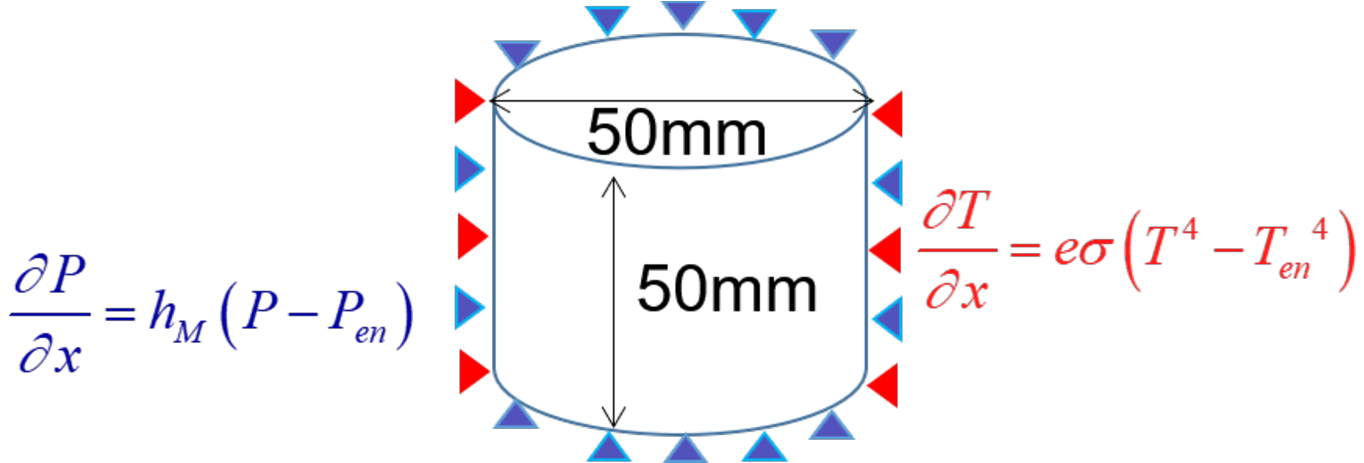
\includegraphics[width=12cm]{./figures/bench_setup.pdf}
	\caption{Geometria, dimensões e condições de contorno utilizadas no {\it benchmark}.
  \label{fig:bench_setup}}
\end{figure}

    \begin{equation}
      \label{eq:mod_phi}
      w(P, T) =
      \begin{cases} 
      w_c \left( \frac{w_0}{c} \ h(P,T) \right)^{\frac{1}{m(T)}} & h(P, T)\leq 0.6 \\
      w_{0.6} + (h(P, T) - 0.6) \frac{(w_{0.85} - w_{0.6})}{(0.85-0.6)} & 0.6 < h(P, T) < 0.85 \\
      w_c \ (0.04 \ (h(P, T) - 0.85) + 0.38 \ (1.1 - \frac{(T - 273.15)^2)}{1.8e5}) & 0.85 \leq h(P, T) 
      \end{cases}
    \end{equation}
 

A Figura \ref{fig:TGA_first} (a) apresenta a comparação entre as temperaturas
medidas pelo termopar próximo a superfície da amostra e as temperaturas da superfície do
modelo. É possível observar que há dois regimes distintos nas amostras aquecidas
à 2$^\degree$C/min e 5$^\degree$C/min. Um primeiro momento no qual
a taxa de aquecimento percebida pela amostra é maior nos dados experimentais do
que os dados do modelo (110 minutos para a amostra aquecida a 2$^\degree$C/min
70 minutos para a 5$^\degree$C/min) e um segundo momento, no qual o cenário se
inverte e a taxa de aquecimento percebida pela superfície da amostra
experimental é menor que a simulada.

\begin{figure}[!ht]
	\centering
	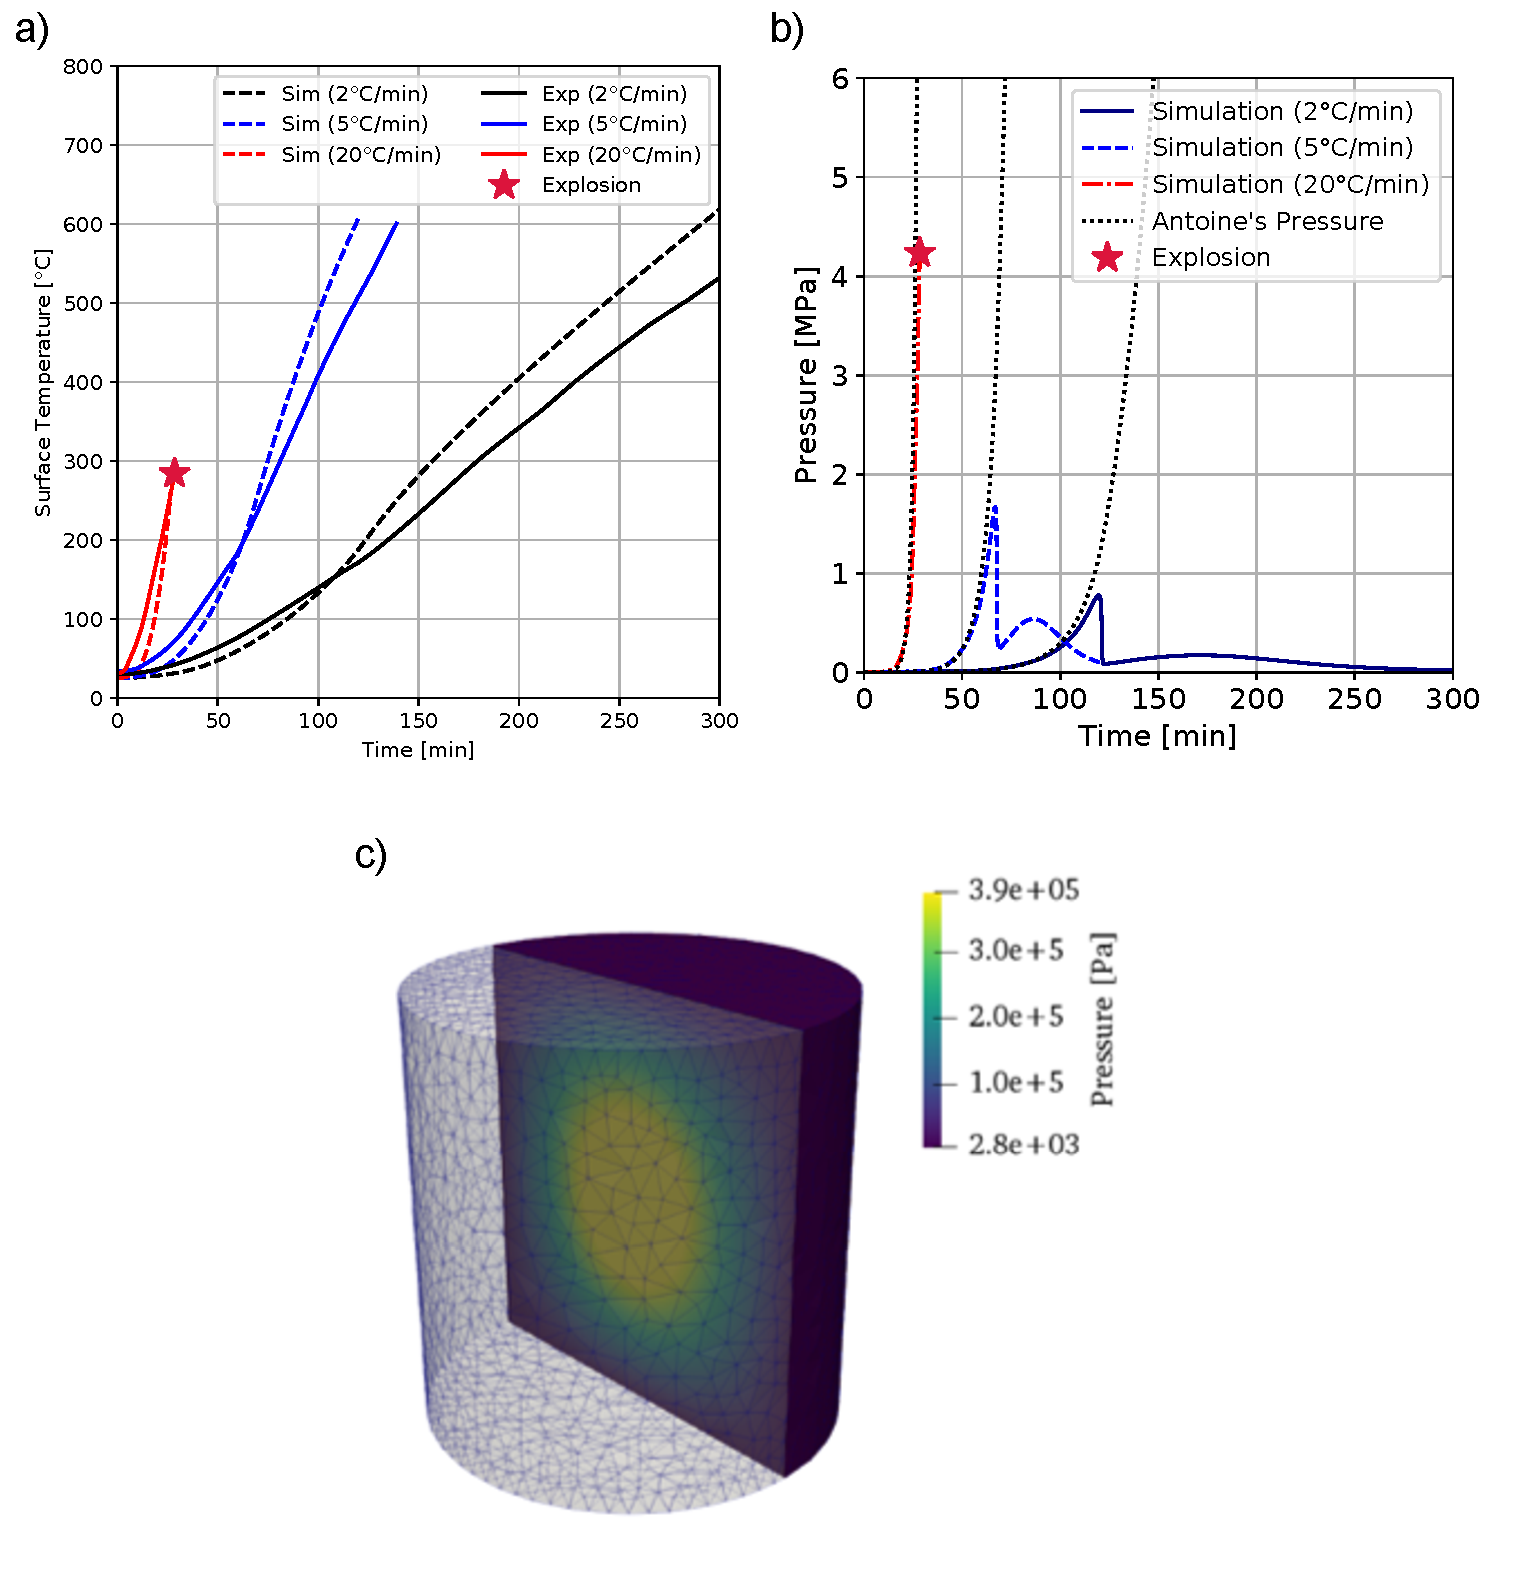
\includegraphics[width=14cm]{./figures/All_TGA_results.pdf}
	\caption{Evolução temporal da temperatura superficial, (a), da pressão máxima
    e da pressão de Antoine (b) e campo escalar de pressões ao final do ensaio da amostra simulada e
    aquecida à 5$^\degree$C/min, (c)).
  \label{fig:TGA_first}}
\end{figure}

Tal momento coincide com o fim da água fisicamente adsorvida, conforme é
possível observar na Figura \ref{fig:TGA_first} (b) que retrata a pressão máxima
em cada incremento de tempo da simulação. Uma vez que o arranjo experimental não
apresenta nenhum transdutor de pressão, tal resultado pode apenas ser comparado
com as curvas de pressão de saturação de Antoine, cujo os valores para a água
são tabelados \cite{yaws2006antoine}. Assim, é possível correlacionar que o fim
da água fisicamente adsorvida reduziu a quantidade de energia térmica necessária
para aumentar a temperatura da amostra fornecida ao sistema. Tal resultado será
referenciado para explicar os resultados seguintes. Por fim, é possível observar
que a amostra aquecida a 20$^\degree$C/min explodiu no momento em que a
simulação previa uma pressão de 4MPa, elevada o suficiente para causar uma
explosão, se estimarmos um módulo de Weibull de 7 e convertermos a resistência
mecânica à flexão três pontos do material (mensurada e valendo 6MPa) para a
resistência mecânica a tração pura (3MPa).

Por fim, a Figura \ref{fig:TGA_first} (c) apresenta todo o campo escalar de
pressões ao final do ensaio da amostra simulada e aquecida à 5$^\degree$C/min,
mostrando que o maior valor de pressão se encontra no centro da amostra.

Em seguida, a Figura \ref{fig:TGA_Mass} apresenta a comparação entre a massa
liberada do ensaio de TGA (curvas em vermelho) e a massa computada pela integral
da quantidade de água evaporável somada à água de desidratação (curva azul
escuro). A princípio é possível observar a mesma transição entre os regimes de
taxas de aquecimento observados nas Figuras \ref{fig:TGA_first} (a) e (b),
ocorrendo sempre a 200$^\degree$C, mostrando que a diferença de tempo entre as amostras
aquecidas a 2$^\degree$C/min e 5$^\degree$C/min é apenas decorrente do intervalo
de tempo necessário para se alcançar a temperatura de 200$^\degree$C.

Embora os resultados demonstrem certa concordância entre a simulação e os dados
experimentais, é possível observar que o ajuste manual da curva de sorção não
representou o comportamento demonstrado nas medidas experimentais, especialmente
da perda de massa em função da temperatura onde se pode ver que na simulação, a
água liberada em baixas temperaturas é muito maior do que a da medida
experimental (especialmente para o caso da amostra aquecida à 20$^\degree$C/min,
curvas vermelhas). 

\begin{figure}[H]
	\centering
	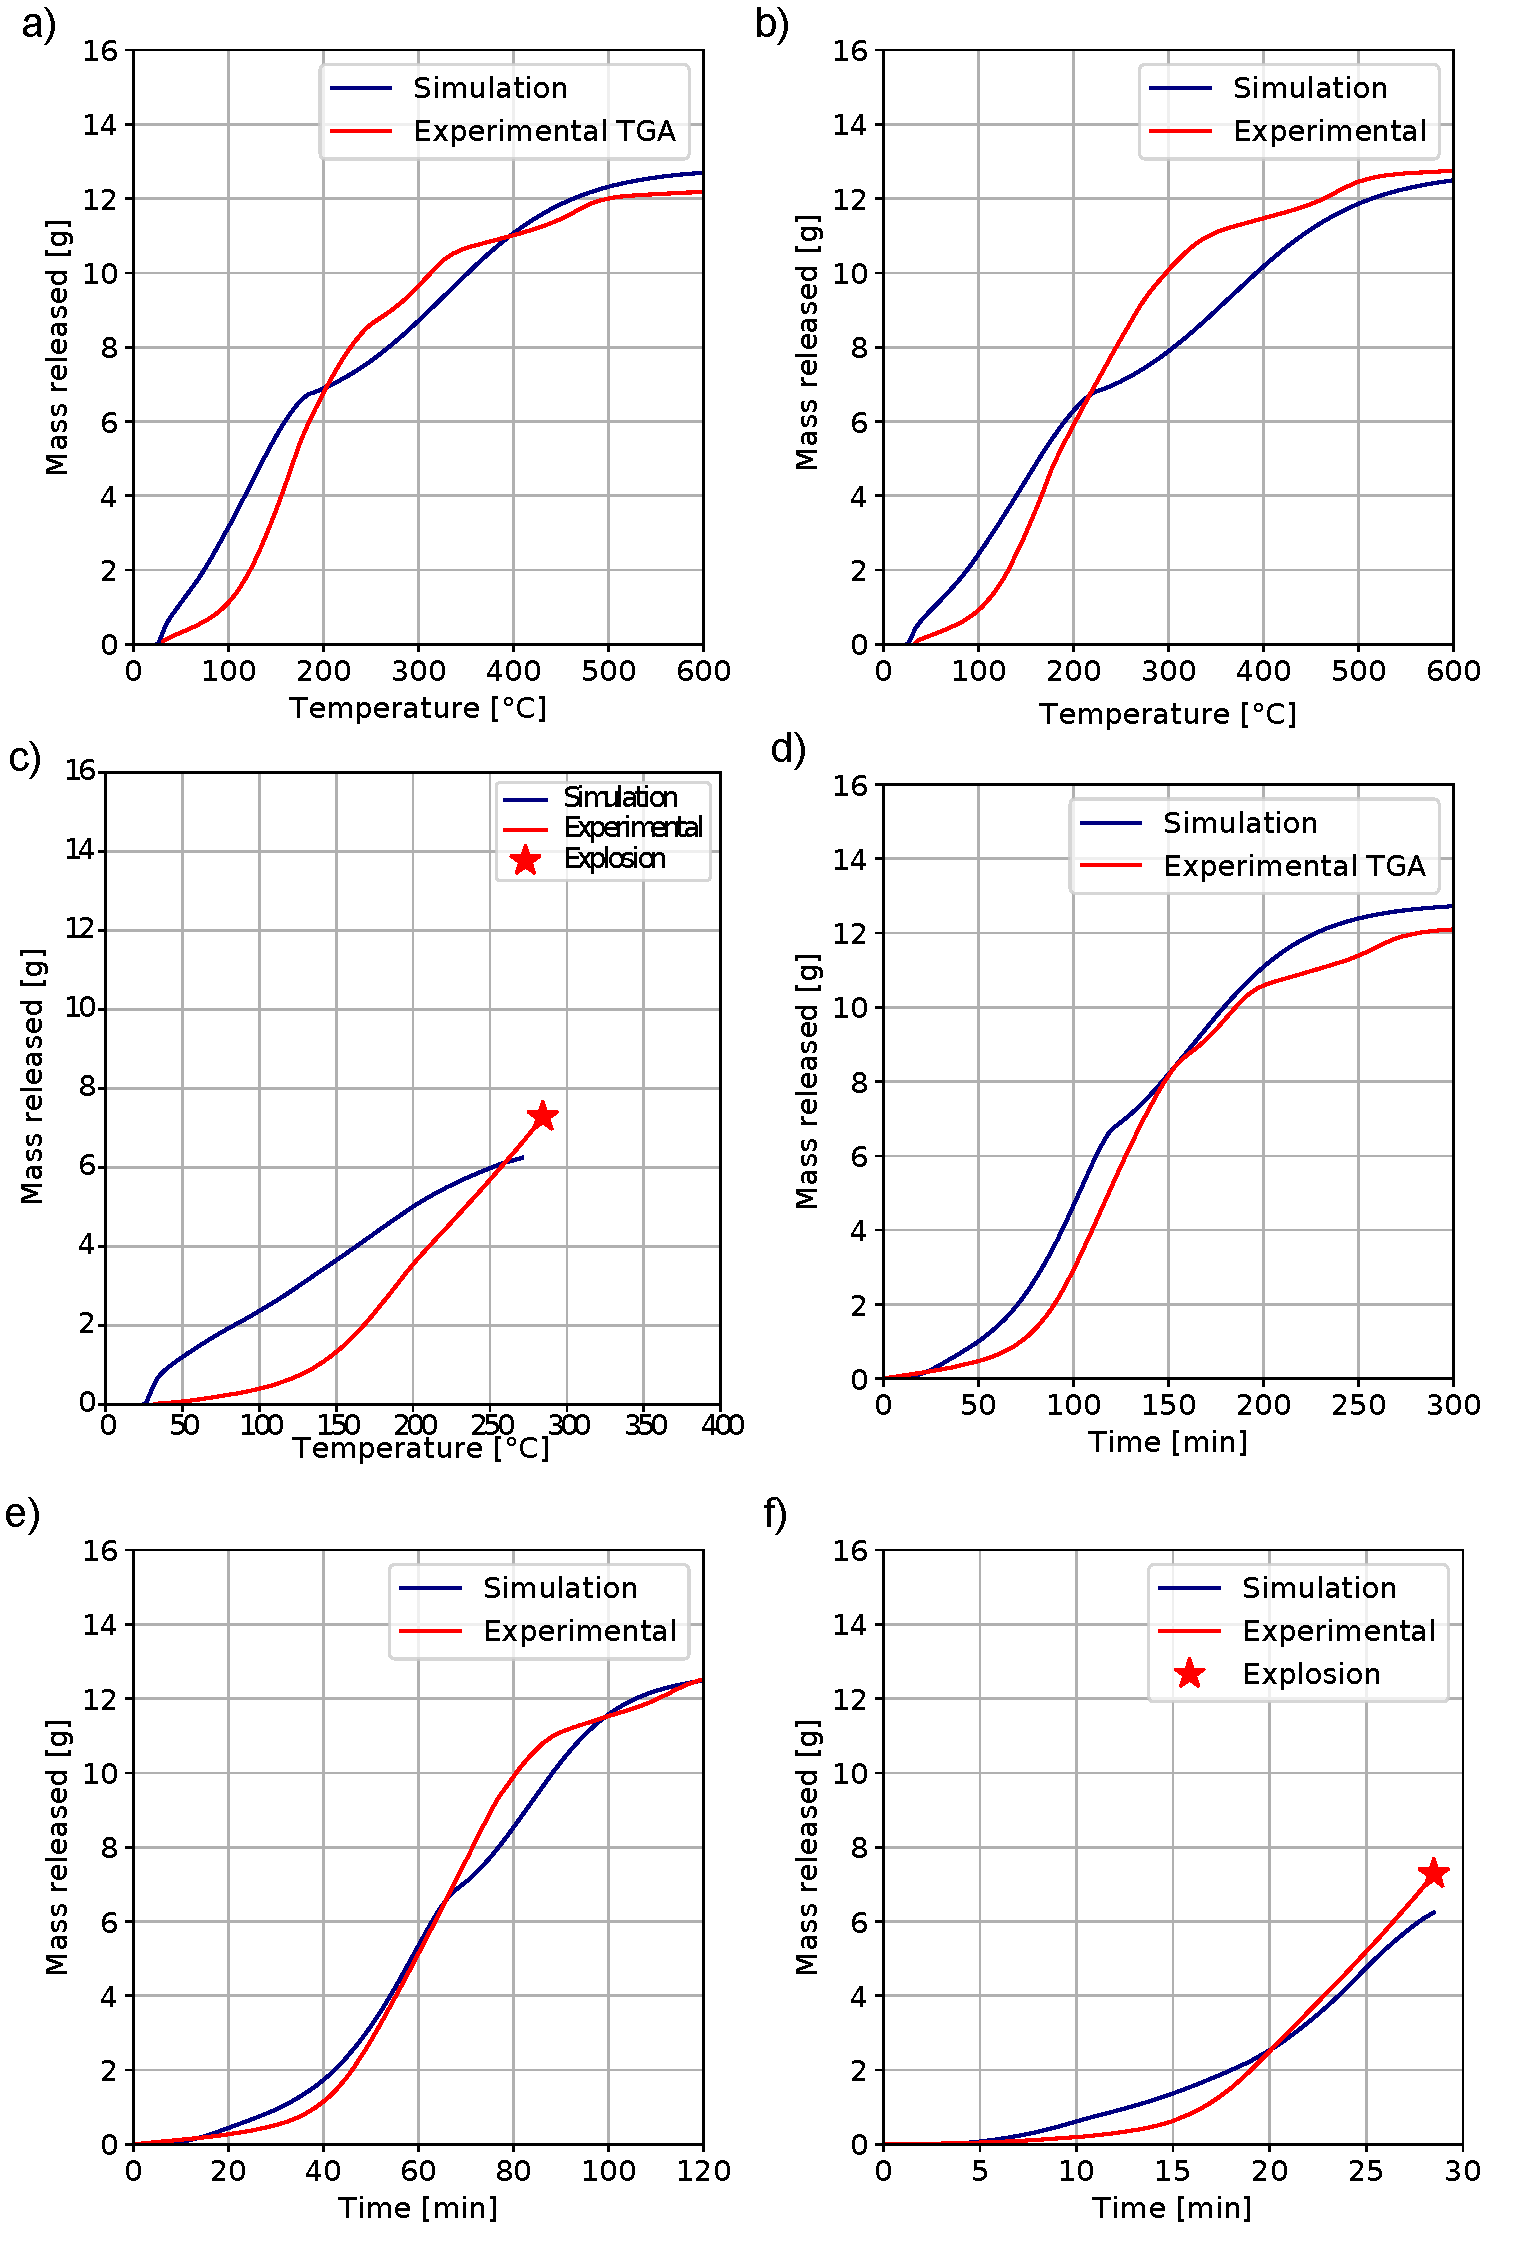
\includegraphics[width=14cm]{./figures/TGA_results_mass.pdf}
	\caption{Resultados de massa liberada em função da temperatura interna, (a),
    (b) e (c), e do tempo de simulação (d), (e) e (f).
  \label{fig:TGA_Mass}}
\end{figure}

\section{Otimização de uma curva de secagem}

A fim de demonstrar o potencial da ferramenta para a otimização da curva de
secagem, um caso fictício será apresentado. Trata-se da simulação da curva de
secagem de uma parede através do aquecimento unidirecional. As propriedades
utilizadas do material foram extraídas de Gong et al, \cite{Gong1995a} e o
modelo é baseado em uma malha unidimensional com 40 elementos lineares. As
condições de contorno são de aquecimento na face esquerda conforme a curva de
secagem, enquanto a face direita é resfriada por convecção natural em um
ambiente à 25$^\degree$C. A amostra é permeável em ambos os lados.

A Figura \ref{fig:No_PID} apresenta a curva de secagem (a), bem como a evolução
da pressão máxima na amostra (b). É possível observar que a pressão máxima
alcança um valor máximo de aproximadamente 10 bar (1.0 MPa, aqui a unidade
escolhida foi bar a fim de facilitar as comparações com o resultados reportados
por Gong) atingida durante o patamar. Tal resultado demonstra que o patamar está
mal dimensionado, uma vez que embora a pressão não cresça no intervalo de 2 a 4
horas, a água não é totalmente retirada, o que leva ao pico no tempo 6h.

\begin{figure}[H]
	\centering
	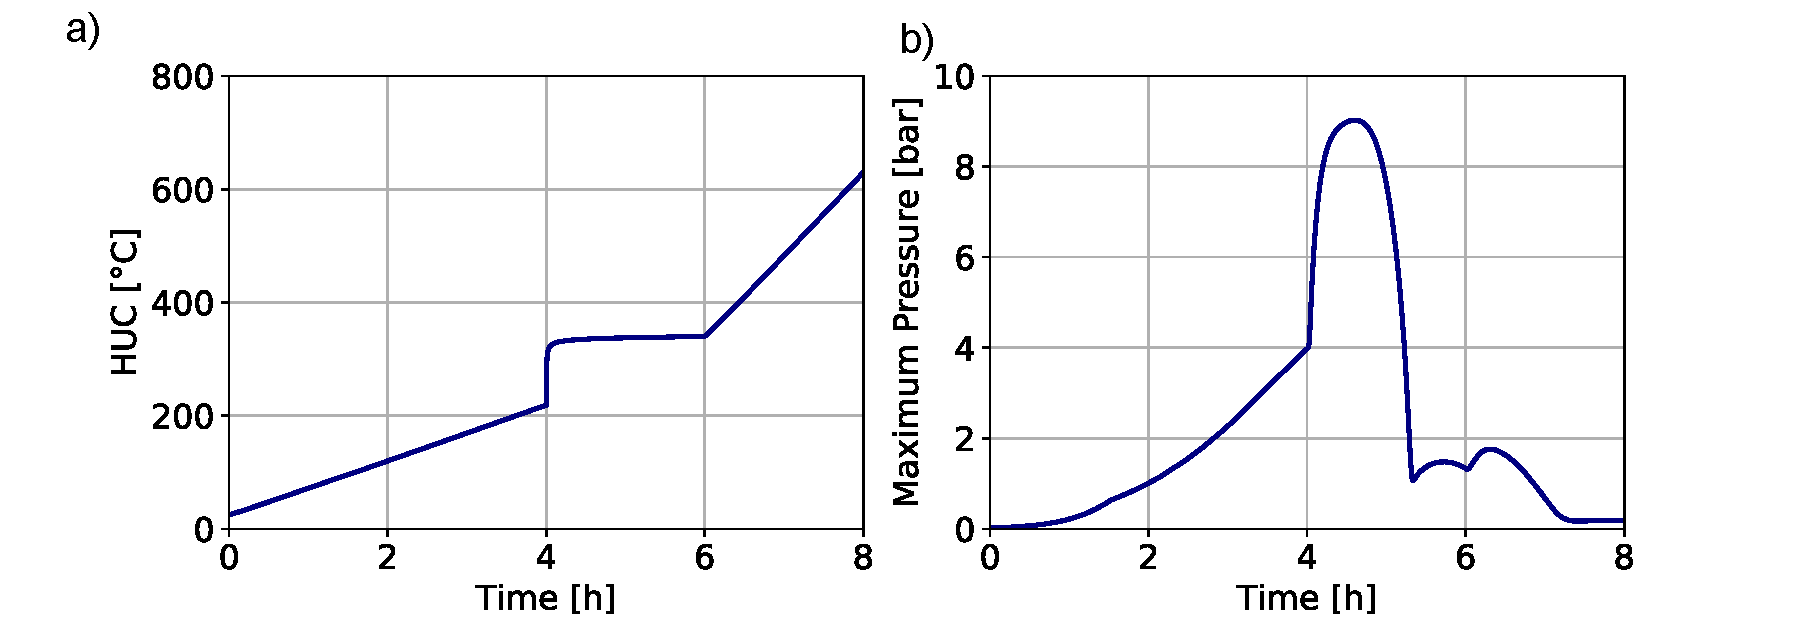
\includegraphics[width=14cm]{./figures/No_PID.pdf}
	\caption{Curva de aquecimento (a) e pressão máxima obtida (b) para o caso de referência.
  \label{fig:No_PID}}
\end{figure}

A fim de propor uma nova curva de secagem, no qual o patamar esteja dimensionado
corretamente, uma abordagem baseada no uso de um controlador do tipo PID,
conforme proposta por Fey et al, \cite{Fey2017c} e descrita na Seção
\ref{mat:pid}, foi utilizada. A pressão limite de 3 bar foi escolhida
arbitrariamente apenas a fim de mostrar o potencial da ferramenta. Como a taxa
de aquecimento do forno apresenta um limite máximo, no presente trabalho foi
necessário adicionar no algoritmo que o máxima taxa de aquecimento fosse de
150$^\degree$C/h (a mesma taxa máxima utilizada no caso anterior, de referência
sem o uso do controlador).


A Figura \ref{fig:PID} (a) apresenta a curva otimizada para a secagem. É
possível observar a existência de um patamar de duas horas na temperatura de
200$^\degree$C, sendo seguido por um forte aquecimento até a secagem completa do
material, conforme mostrado pela curva de pressão máxima (b). Também é possível
observar em (c) que o aquecimento da temperatura ambiente até 200$^\degree$C naõ foi
realizado a uma taxa constante, mas sim com uma taxa decrescente, de modo que a
pressão não excedesse tanto o limite de controle. Aqui é possível observar que o
algoritmo utilizado pelo controlador apresenta um {\it overshoot} de 1 bar
(conforme evidenciado em (d)).

A presença de tal fenômeno se explica pelo caráter dinâmico do problema, havendo
uma certa inércia entre a atuação do controlador e o seu efeito na resposta. Fey
et al, no trabalho referenciado resolveu tal problemática ao fazer uso de um
segundo loop de controle, adicionando um termo de erro proporcional à posição da
pressão máxima, de forma que fosse compensada e antecipada a ocorrência de {\it
  overshootings}.

\begin{figure}[H]
	\centering
	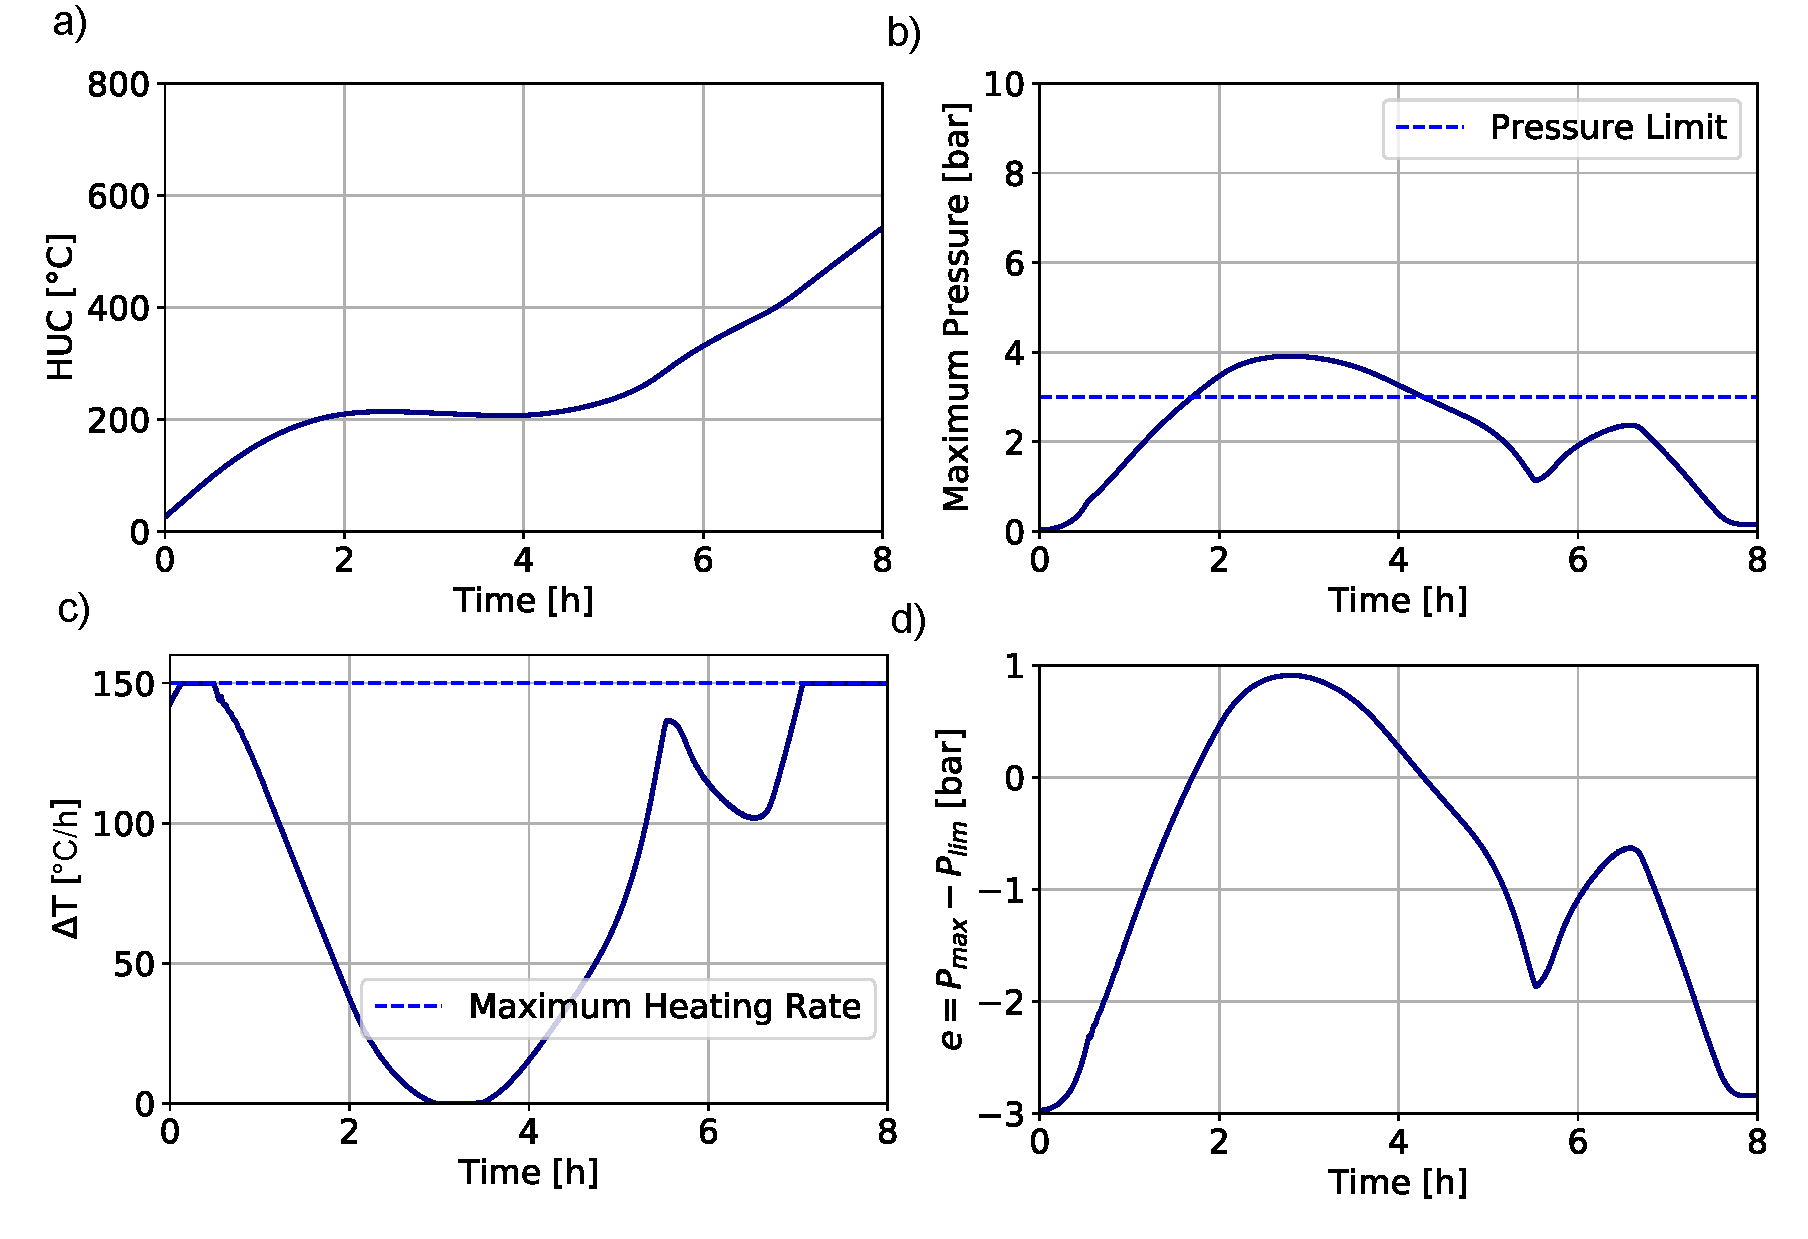
\includegraphics[width=14cm]{./figures/PID.pdf}
	\caption{Resultados de massa liberada em função da temperatura interna, (a),
    (b).
  \label{fig:PID}}
\end{figure}

No presente trabalho, tal estrutura complexa de algoritmo não foi contemplada
devido a limitações no tempo de desenvolvimento, e devido a possibilidade de já
se propor a ferramenta atual como uma solução tecnológica desde que a pressão
limite seja ajustada a fim de evitar que o {\it overshoot} supere os limites de
segurança.

Além disso, a fim de se aplicar tal curva de aquecimento, as limitações dos
controladores dos queimadores industriais faria necessário uma etapa de
simplificação da curva de secagem otimizada encontrada na Figura \ref{fig:PID}
a), a fim de que está tivesse apenas taxas constantes de aquecimento. A
comparação entre a curva de secagem otimizada original e a simplificada poderia
ser feita pelo próprio modelo garantindo assim que mesmo tendo este formato mais
simples, ela ainda funcionaria em manter as pressões no interior do material
controladas.

%%% Local Variables:
%%% mode: latex
%%% TeX-master: "TCC-Secagem"
%%% End:
